% !TeX root = ../../../main.tex
\begin{figure}[htbp]
\begin{ChSixFloatBody}

\centering
    \begin{minipage}[t]{0.3\textwidth}
    \centering
    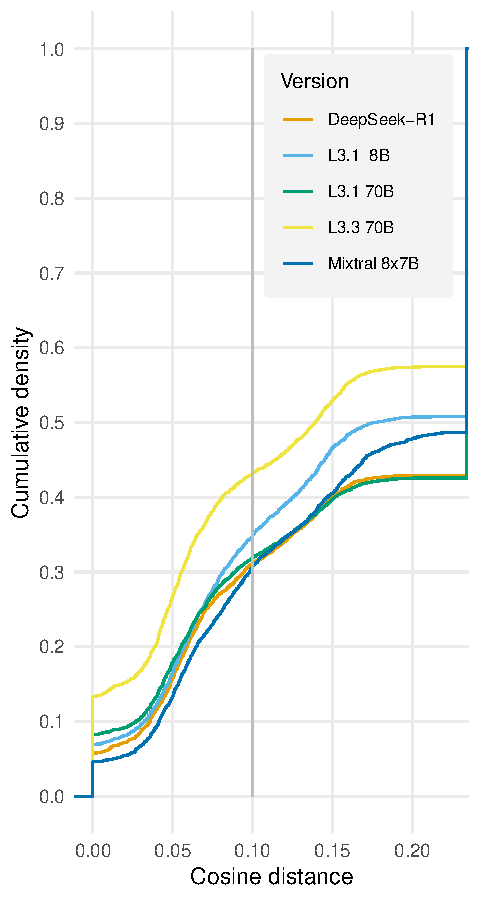
\includegraphics[width=\linewidth, page=1]{Appendices/appendix-ch06/images/figures/main_results_figures/figures_i2m4.pdf}
    \end{minipage}
% \end{figure}
    % \hfill
    \begin{minipage}[t]{0.3\textwidth}
% \begin{figure}[h!]j
    \centering
    \includegraphics[width=\linewidth, page=2]{Appendices/appendix-ch06/images/figures/main_results_figures/figures_i2m4.pdf}
    \end{minipage}
    % \caption{Event match cumulative distribution function (left) and  concordance box-plots (right) for the \texttt{sepsis-40} dataset.}
    % \label{fig:sep10eventc}
% \end{figure}
% \begin{figure}[tb!]

    \begin{minipage}[t]{0.3\textwidth}
    \centering
    \includegraphics[width=\linewidth, page=3]{Appendices/appendix-ch06/images/figures/main_results_figures/figures_i2m4.pdf}
    \end{minipage}
% \end{figure}
% \begin{figure}[h!]
    \begin{minipage}[t]{0.3\textwidth}
    \centering
    \includegraphics[width=\linewidth, page=4]{Appendices/appendix-ch06/images/figures/main_results_figures/figures_i2m4.pdf}
    \end{minipage}
    
    

\end{ChSixFloatBody}
\caption{Event match cumulative distribution function (top left) and  concordance box-plots (top right) for the i2m4 dataset. 
    Time discrepancy from the manual annotation timestamps among matched events, overall (bottom left) and disaggregated by clinician annotator timestamp (time from presentation, bottom right).}\ChSixFloatLabel{ch06:fig:i2m4-time-disc}
\end{figure}